% Intestazione
\fancyhead[L]{3 \hspace{0.2cm} Casi d'uso} % Testo a sinistra

\setcounter{secnumdepth}{5} % Per il 5° livello di sezione


\section{Casi d'uso}
\label{sec:casi_uso}

\subsection{Scopo}

Lo scopo di questa sezione è descrivere in maniera dettagliata i casi d’uso individuati dal
gruppo, in riferimento alle funzionalità dell’applicazione.


\subsection{Attori}

L’applicazione prevede la presenza di \dots


\subsection{Lista casi d'uso}




% TEMPLATE

\begin{comment}
\hypertarget{UC0}{}
\subsubsection{UC0: \dots}

\begin{figure}[h]
    \centering
    
\includegraphics[width=\textwidth]{placeholder.png}
    \caption{\dots}
\end{figure}

\begin{itemize}
    \item \textbf{Attori principali}: \dots;
    \item \textbf{Precondizioni}: \dots;
    % Oppure, se ci sono più precondizioni:
    \item \textbf{Precondizioni}: 
    \begin{itemize}
        \item \dots;
        \item \dots.
    \end{itemize}
    \item \textbf{Trigger}: \dots;
    \item \textbf{Postcondizioni}: \dots;
    \item \textbf{Scenario principale}:
    \begin{enumerate}
        \item \dots;
        \item \dots.
    \end{enumerate}
    \item \textbf{Sottocasi d'uso}:
    \begin{itemize}
        \item \dots;
        \item \dots.
    \end{itemize}
    \item \textbf{Scenario alternativo}:
    \begin{enumerate}
        \item \dots;
        \item \dots.
    \end{enumerate}
\end{itemize}
\end{comment}




\hypertarget{UC1}{}
\subsubsection{UC1: Inserimento di interrogazione in linguaggio naturale}

\begin{figure}[h]
    \centering
    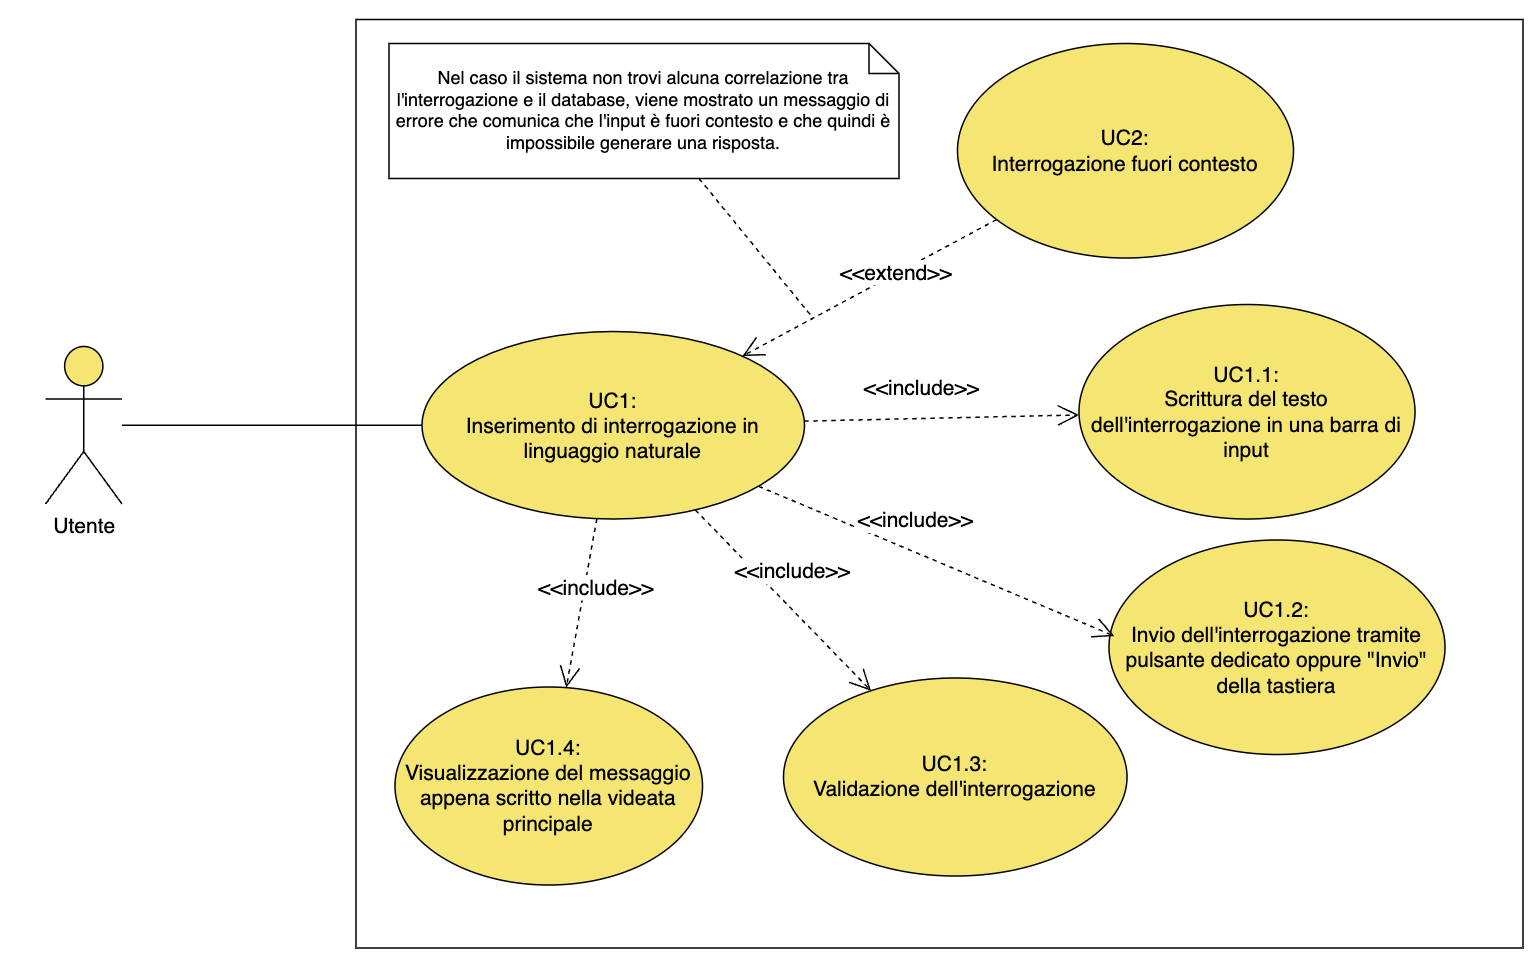
\includegraphics[width=\textwidth]{Diagramma UC1 - UC2.png}
    \caption{Inserimento di interrogazione in linguaggio naturale}
\end{figure}

\begin{itemize}
    \item \textbf{\emph{Attori}\textsubscript{\textbf{\textit{G}}} principali}: Utente;
    \item \textbf{Precondizioni}: L'utente deve avere accesso all'interfaccia dell'applicazione connessa al database;
    \item \textbf{\emph{Trigger}\textsubscript{\textbf{\textit{G}}}}: L'utente desidera inserire un'interrogazione in linguaggio naturale nella barra di input;
    \item \textbf{Postcondizioni}: L'interrogazione viene inviata e, se valida, genera una risposta adeguata. Se non valida, l'utente riceve un messaggio di errore;
    \item \textbf{\emph{Scenario principale}\textsubscript{\textbf{\textit{G}}}}:
    \begin{enumerate}
        \item L'utente accede all'interfaccia dell'applicazione;
        \item \bulhyperlink{UC1.1}{UC1.1}: L'utente scrive l'interrogazione in linguaggio naturale nella barra di input.
        \item \bulhyperlink{UC1.3}{UC1.3}: Il sistema valida l'interrogazione.
        \item \bulhyperlink{UC1.4}{UC1.4}: Il sistema mostra il messaggio generato nella schermata principale.
    \end{enumerate}
    \item \textbf{\emph{Sottocasi d'uso}\textsubscript{\textbf{\textit{G}}}}:
    \begin{itemize}
        \item \bulhyperlink{UC1.1}{UC1.1}: L'utente scrive l'interrogazione in linguaggio naturale nella barra di input.
        \item \bulhyperlink{UC1.2}{UC1.2}: L'utente invia l'interrogazione tramite il pulsante dedicato o "Invio" dalla tastiera.
        \item \bulhyperlink{UC1.3}{UC1.3}: Il sistema valida l'interrogazione.
        \item \bulhyperlink{UC1.4}{UC1.4}: Il sistema mostra il messaggio generato nella schermata principale.
    \end{itemize}
    \item \textbf{\emph{Scenario alternativo}\textsubscript{\textbf{\textit{G}}}}:
    \begin{enumerate}
        \item \bulhyperlink{UC2}{UC2}: Viene inviato un messaggio all'utente che comunica che l'input è fuori contesto e che quindi non è possibile generare una risposta;
        \item \bulhyperlink{UC6}{UC6}: Pur riconoscendo il contesto corretto, il sistema non trova una correlazione tra l'interrogazione e il database, e allora viene visualizzata una risposta negativa.
    \end{enumerate}
\end{itemize}

\hypertarget{UC1.1}{}
\subsubsubsection{UC1.1: Scrittura del testo dell'interrogazione in una barra di input}
\begin{itemize}
    \item \textbf{Attori principali}: Utente;
    \item \textbf{Precondizioni}: L'utente deve avere accesso all'interfaccia dell'applicazione connessa al database;
    \item \textbf{Trigger}: L'utente desidera inserire un'interrogazione in linguaggio naturale;
    \item \textbf{Postcondizioni}: L'utente è riuscito ad inserire l'interrogazione in linguaggio naturale;
    \item \textbf{Scenario principale}:
    \begin{enumerate}
        \item L'utente deve avere accesso all'interfaccia dell'applicazione connessa al database;
        \item L'utente inserisce un'interrogazione in linguaggio naturale.
    \end{enumerate}
\end{itemize}

\hypertarget{UC1.2}{}
\subsubsubsection{UC1.2: Invio dell'interrogazione tramite pulsante dedicato oppure "Invio" della tastiera}
\begin{itemize}
    \item \textbf{Attori principali}: Utente;
    \item \textbf{Precondizioni}: L'utente è riuscito ad inserire l'interrogazione in linguaggio naturale;
    \item \textbf{Trigger}: L'utente desidera inviare l'interrogazione tramite il pulsante dedicato oppure "Invio" della tastiera;
    \item \textbf{Postcondizioni}: L'interrogazione è stata inviata;
    \item \textbf{Scenario principale}:
    \begin{enumerate}
        \item \bulhyperlink{UC1.1}{UC1.1}: L'utente è riuscito ad inserire l'interrogazione in linguaggio naturale;
        \item Invio dell'interrogazione tramite pulsante dedicato oppure "Invio" della tastiera;
        \item L'interrogazione è stata inviata.
    \end{enumerate}
\end{itemize}

\hypertarget{UC1.3}{}
\subsubsubsection{UC1.3: Validazione dell'interrogazione}
\begin{itemize}
    \item \textbf{Attori principali}: Utente;
    \item \textbf{Precondizioni}: L'interrogazione è stata inviata;
    \item \textbf{Trigger}: L'utente desidera sapere se l'interrogazione che ha scritto è valida;
    \item \textbf{Postcondizioni}: Visualizzazione del messaggio appena scritto nella videata principale;
    \item \textbf{Scenario principale}:
    \begin{enumerate}
        \item \bulhyperlink{UC1.2}{UC1.2}: L'interrogazione è stata inviata;
        \item L'interrogazione viene validata;
        \item \bulhyperlink{UC1.4}{UC1.4}: Visualizzazione del messaggio appena scritto nella videata principale.
    \end{enumerate}
\end{itemize}

\hypertarget{UC1.4}{}
\subsubsubsection{UC1.4: Visualizzazione del messaggio appena scritto nella videata principale}
\begin{itemize}
    \item \textbf{Attori principali}: Utente;
    \item \textbf{Precondizioni}: L'interrogazione deve essere valida;
    \item \textbf{Trigger}: L'utente desidera visualizzare il messaggio appena scritto nella videata principale;
    \item \textbf{Postcondizioni}: L'utente visualizza sullo schermo il messaggio;
    \item \textbf{Scenario principale}:
    \begin{enumerate}
        \item \bulhyperlink{UC1.3}{UC1.3}: L'interrogazione è stata validata;
        \item L'interrogazione viene visualizzata sullo schermo.
    \end{enumerate}
\end{itemize}


\hypertarget{UC2}{}
\subsubsection{UC2: Interrogazione fuori contesto}

\begin{itemize}
    \item \textbf{Attori principali}: Utente;
    \item \textbf{Precondizioni}: L'utente ha inserito un'interrogazione in linguaggio naturale;
    \item \textbf{Trigger}: L'utente desidera ricevere informazioni legate esclusivamente ai contenuti del database associato al sistema;
    \item \textbf{Postcondizioni}: Viene visualizzato un messaggio che comunica all'utente che l'input è fuori contesto e che quindi è impossibile generare una risposta;
    \item \textbf{Scenario principale}:
    \begin{enumerate}
        \item Il sistema analizza la frase e cerca di contestualizzarla utilizzando i dati presenti nel database;
        \item Il sistema rileva che la frase è fuori contesto e non può essere associata a nessuna informazione rilevante nel database;
        \item Il sistema invia un messaggio all'utente indicando che la frase è fuori contesto e richiede ulteriori chiarimenti.
    \end{enumerate}
\end{itemize}
\newpage


\hypertarget{UC3}{}
\subsubsection{UC3: Generazione della risposta}

\begin{figure}[h]
    \centering
    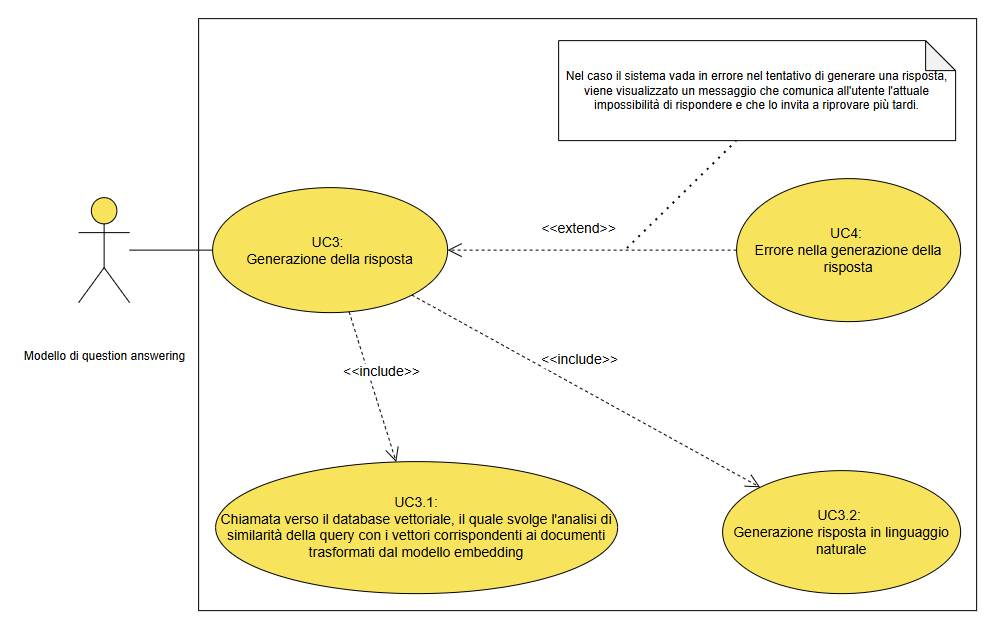
\includegraphics[width=\textwidth]{Diagramma UC3 - UC4.png}
    \caption{Generazione della risposta}
\end{figure}

\begin{itemize}
    \item \textbf{Attori principali}: Modello di question answering;
    \item \textbf{Precondizioni}: Il modelo di embedding e il database vettoriale devono essere funzionanti e reperibili;
    \item \textbf{Trigger}: Una domanda è stata inviata;
    \item \textbf{Postcondizioni}: Se la risposta viene generata, l'utente visualizza la risposta. Se invece si genera un errore, viene visualizzato un messaggio che lo riporta;
    \item \textbf{Scenario principale}:
    \begin{enumerate}
        \item La domanda viene inviata.
        \item \bulhyperlink{UC3.1}{UC3.1}: Il database vettoriale si occupa di trovare i documenti inerenti alla domanda;
        \item \bulhyperlink{UC3.2}{UC3.2}: L'LLM genera la risposta utilizzando la domanda e tutti i documenti inerenti;
    \end{enumerate}
    \item \textbf{Sottocasi d'uso}:
    \begin{itemize}
        \item \bulhyperlink{UC3.1}{UC3.1}: tramite la domanda il database vettoriale cerca, nei documenti trasformati dal modello di embedding, similarità trovando i documenti inerenti;
        \item \bulhyperlink{UC3.2}{UC3.2}: L'LLM genera una risposta basata sul prompt iniziale, e i documenti inerenti trovati dal database vettoriale;
    \end{itemize}
    \item \textbf{Scenario alternativo}:
    \begin{enumerate}
        \item \bulhyperlink{UC4}{UC4}: Viene inviato un messaggio all'utente che comunica un errore durante la generazione della risposta;
    \end{enumerate}
\end{itemize}

\hypertarget{UC3.1}{}
\subsubsubsection{UC3.1: Ricerca dei dati inerenti alla domanda tramite database vettoriale}
\begin{itemize}
    \item \textbf{Attori principali}: Database vettoriale;
    \item \textbf{Precondizioni}: Il modelo di embedding ed il database vettoriale devono essere funzionanti e reperibili;
    \item \textbf{Trigger}: Una domanda è stata inviata;
    \item \textbf{Postcondizioni}: vengono restituiti i documenti ritenuti rilevanti se presenti;
    \item \textbf{Scenario principale}:
    \begin{enumerate}
        \item La domanda viene confrontata, tramite il database vettoriale, ai documenti processati dal modello di embedding;
        \item Vengono restituiti i documenti inerenti.
    \end{enumerate}
\end{itemize}

\hypertarget{UC3.2}{}
\subsubsubsection{UC3.2: Generazione della risposta in linguaggio naturale}
\begin{itemize}
    \item \textbf{Attori principali}: LLM;
    \item \textbf{Precondizioni}: La domanda è stata processata dal database vettoriale;
    \item \textbf{Trigger}: Fine ricerca di dati rilevanti alla domanda;
    \item \textbf{Postcondizioni}: La risposta in linguaggio naturale è stata generata;
    \item \textbf{Scenario principale}:
    \begin{enumerate}
        \item \bulhyperlink{UC3.1}{UC3.1}: Vengono restituiti i documenti inerenti alla domanda;
        \item L'LLM genera la risposta in linguaggo naturale prendendo in considerazione la domanda e i documenti inerenti;
        \item La risposta viene generata.
    \end{enumerate}
\end{itemize}

\hypertarget{UC4}{}
\subsubsection{UC4: Errore nella generazione della risposta}

\begin{itemize}
    \item \textbf{Attori principali}: Modello di question answering;
    \item \textbf{Precondizioni}: Il modelo di embedding e il database vettoriale devono essere funzionanti e reperibili;
    \item \textbf{Trigger}: Una domanda è stata inviata;
    \item \textbf{Postcondizioni}: Viene visualizzato un messaggio di errore, chiedendo di riprovare più tardi;
    \item \textbf{Scenario principale}:
    \begin{enumerate}
        \item La domanda viene inviata;
        \item Si genera un errore durante il processo che non permette la generazione della risposta;
        \item Viene visualizzato il messaggio di errore.
    \end{enumerate}
\end{itemize}


\hypertarget{UC5}{}
\subsubsection{UC5: Visualizzazione della risposta generata}

\begin{figure}[h]
    \centering
    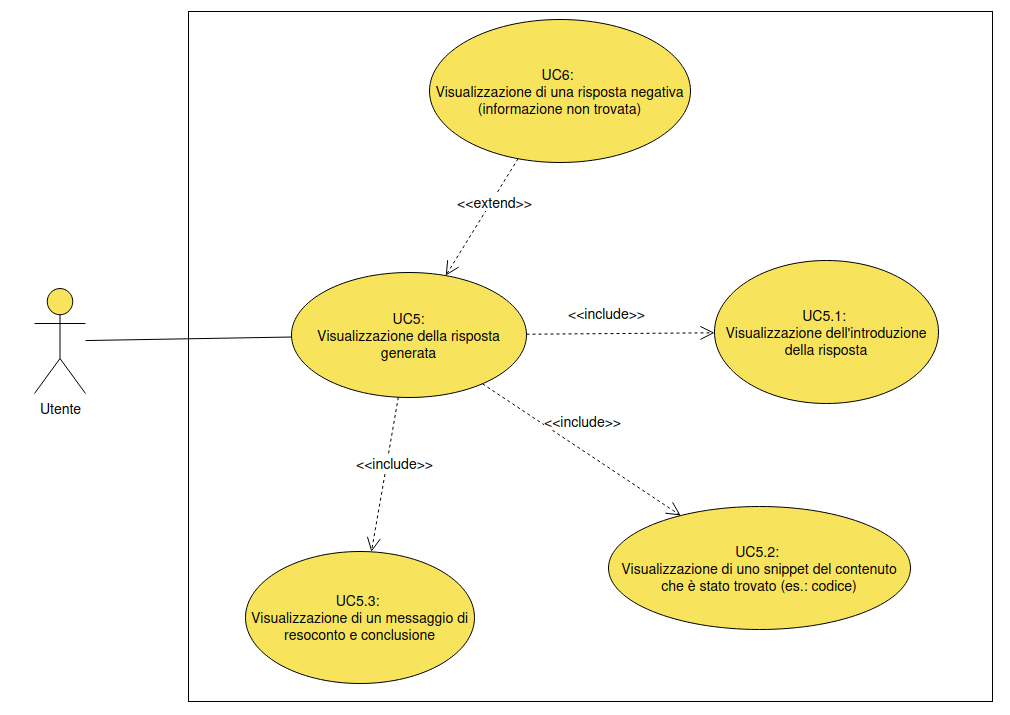
\includegraphics[width=\textwidth]{Diagramma UC5 - UC6.png}
    \caption{Visualizzazione della risposta generata}
\end{figure}

\begin{itemize}
    \item \textbf{Attori principali}: Utente;
    \item \textbf{Precondizioni}: Il sistema ha generato correttamente la risposta alla domanda dell'utente;
    \item \textbf{Trigger}: L'utente desidera visualizzare la risposta alla domanda che ha posto;
    \item \textbf{Postcondizioni}: L'utente visualizza la risposta generata dal sistema;
    \item \textbf{Scenario principale}:
    \begin{enumerate}
        \item \bulhyperlink{UC3}{UC3}: Il sistema ha generato correttamente la risposta alla domanda dell'utente;
        \item L'utente visualizza la risposta generata dal sistema.
    \end{enumerate}
    \item \textbf{Sottocasi d'uso}:
    \begin{itemize}
        \item \bulhyperlink{UC5.1}{UC5.1}: Visualizzazione dell'introduzione della risposta;
        \item \bulhyperlink{UC5.2}{UC5.2}: Visualizzazione di uno \emph{snippet}\textsubscript{\textbf{\textit{G}}} del contenuto che è stato trovato (es.: codice);
        \item \bulhyperlink{UC5.3}{UC5.3}: Visualizzazione di un messaggio di resoconto e conclusione.
    \end{itemize}
    \item \textbf{Scenario alternativo}:
    \begin{enumerate}
        \item \bulhyperlink{UC6}{UC6}: Visualizzazione di una risposta negativa (informazione non trovata).
    \end{enumerate}
\end{itemize}



\hypertarget{UC5.1}{}
\subsubsubsection{UC5.1: Visualizzazione dell'introduzione della risposta}

\begin{itemize}
    \item \textbf{Attori principali}: Utente;
    \item \textbf{Precondizioni}: Il sistema ha generato correttamente la risposta alla domanda dell'utente;
    \item \textbf{Trigger}: L'utente desidera visualizzare l'introduzione della risposta alla domanda che ha posto;
    \item \textbf{Postcondizioni}: L'utente visualizza l'introduzione della risposta generata dal sistema;
    \item \textbf{Scenario principale}:
    \begin{enumerate}
        \item \bulhyperlink{UC3}{UC3}: Il sistema ha generato correttamente la risposta alla domanda dell'utente;
        \item L'utente visualizza l'introduzione della risposta generata dal sistema.
    \end{enumerate}
\end{itemize}



\hypertarget{UC5.2}{}
\subsubsubsection{UC5.2: Visualizzazione di uno snippet del contenuto che è stato trovato (es.: codice)}

\begin{itemize}
    \item \textbf{Attori coinvolti}: Utente;
    \item \textbf{Precondizioni}: 
    \begin{itemize}
        \item L'utente ha visualizzato l'introduzione della risposta generata dal sistema;
        \item La risposta generata dal sistema contiene uno snippet di codice.
    \end{itemize}
    \item \textbf{Trigger}: L'utente desidera visualizzare lo snippet di codice contenuto nella risposta alla domanda che ha posto;
    \item \textbf{Postcondizioni}: L'utente visualizza uno snippet di codice contenuto della risposta generata dal sistema;
    \item \textbf{Scenario principale}:
    \begin{enumerate}
        \item \bulhyperlink{UC5.1}{UC5.1}: L'utente ha visualizzato l'introduzione della risposta generata dal sistema;
        \item L'utente visualizza uno snippet del contenuto che è stato trovato (es.: codice).
    \end{enumerate}
\end{itemize}



\hypertarget{UC5.3}{}
\subsubsubsection{UC5.3: Visualizzazione di un messaggio di resoconto e conclusione}

\begin{itemize}
    \item \textbf{Attori coinvolti}: Utente;
    \item \textbf{Precondizioni}: L'utente ha visualizzato almeno l'introduzione della risposta generata dal sistema;
    \item \textbf{Trigger}: L'utente desidera visualizzare la conclusione della risposta alla domanda che ha posto;
    \item \textbf{Postcondizioni}: L'utente visualizza un messaggio di resoconto e conclusione contenuto nella risposta generata dal sistema;
    \item \textbf{Scenario principale}:
    \begin{enumerate}
        \item \bulhyperlink{UC5.1}{UC5.1}: L'utente ha visualizzato l'introduzione della risposta generata dal sistema;
        \item \bulhyperlink{UC5.2}{UC5.2}: Se presente, l'utente ha visualizzato lo snippet di codice contenuto nella risposta;
        \item L'utente visualizza un messaggio di resoconto e conclusione che termina la risposta.
    \end{enumerate}
\end{itemize}



\hypertarget{UC6}{}
\subsubsection{UC6: Visualizzazione di una risposta negativa (informazione non trovata)}

\begin{itemize}
    \item \textbf{Attori coinvolti}: Utente;
    \item \textbf{Precondizioni}: Il sistema non ha trovato nei documenti di contesto l'informazione che l'utente ha domandato;
    \item \textbf{Trigger}: L'utente desidera visualizzare la risposta alla domanda che ha posto;
    \item \textbf{Postcondizioni}: L'utente visualizza come risposta un messaggio del sistema in cui gli viene segnalata la mancanza dell'informazione 
    richiesta nei dati forniti come contesto;
    \item \textbf{Scenario principale}:
    \begin{enumerate}
        \item Il sistema non ha trovato nei documenti di contesto l'informazione che l'utente ha domandato;
        \item L'utente visualizza come risposta un messaggio del sistema in cui gli viene segnalata la mancanza dell'informazione richiesta 
        nei dati forniti come contesto.
    \end{enumerate}
\end{itemize}






\hypertarget{UC8}{}
\subsubsection{UC8: Visualizzare una risposta generata con dati di contesto provenienti da 
\emph{GitHub}\textsubscript{\textbf{\textit{G}}}, \emph{Jira}\textsubscript{\textbf{\textit{G}}} e 
\emph{Confluence}\textsubscript{\textbf{\textit{G}}}}






\hypertarget{UC11}{}
\subsubsection{UC11: Visualizzazione di una risposta generata utilizzando dati di contesto aggiornati}

\begin{figure}[h]
    \centering
    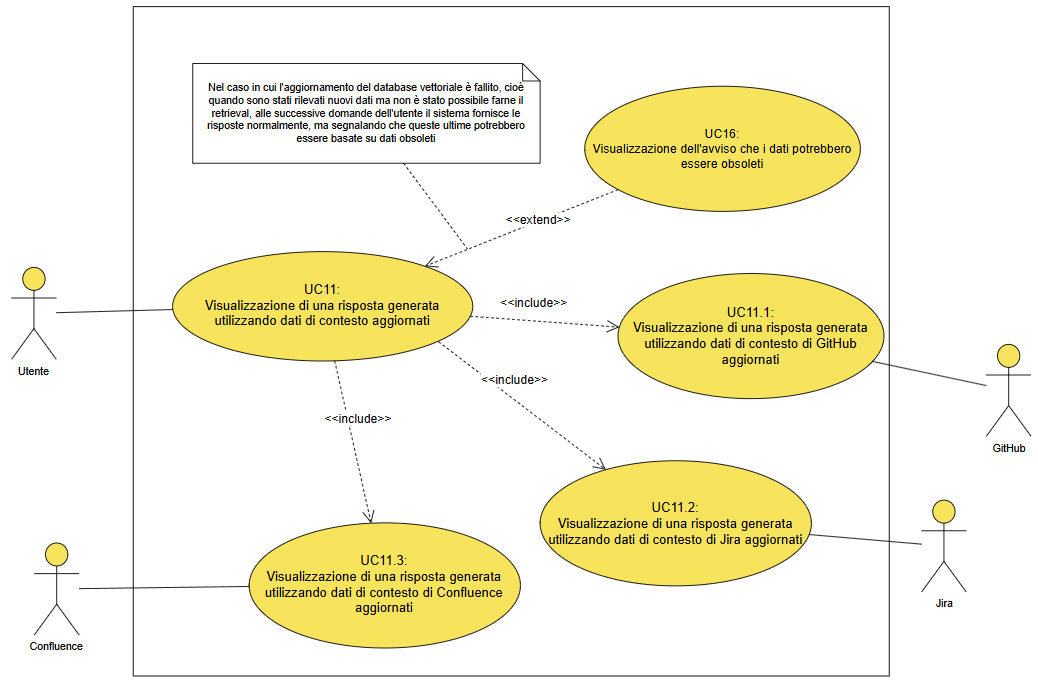
\includegraphics[width=\textwidth]{Diagramma UC11 - UC16.png}
    \caption{Visualizzazione di una risposta generata utilizzando dati di contesto aggiornati}
\end{figure}

\begin{itemize}
    \item \textbf{Attori principali}: Utente;
    \item \textbf{Precondizioni}: 
    \begin{itemize}
        \item L'utente ha inserito una interrogazione in linguaggio naturale;
        \item Il sistema ha generato correttamente la risposta alla domanda dell'utente.
    \end{itemize}
    \item \textbf{Trigger}: L'utente desidera visualizzare una risposta basata su dati aggiornati alla domanda che ha posto;
    \item \textbf{Postcondizioni}: L'utente visualizza una risposta generata su dati di contesto aggiornati;
    \item \textbf{Scenario principale}:
    \begin{enumerate}
        \item \bulhyperlink{UC1}{UC1}: L'utente ha inserito una interrogazione in linguaggio naturale;
        \item \bulhyperlink{UC3}{UC3}: Il sistema ha generato correttamente la risposta alla domanda dell'utente;
        \item La risposta è stata generata basandosi su dati aggiornati;
        \item \bulhyperlink{UC5}{UC5}: L'utente visualizza la risposta.
    \end{enumerate}
    \item \textbf{Sottocasi d'uso}:
    \begin{itemize}
        \item \bulhyperlink{UC11.1}{UC11.1}: Visualizzazione di una risposta generata utilizzando dati di contesto di 
        GitHub aggiornati;
        \item \bulhyperlink{UC11.2}{UC11.2}: Visualizzazione di una risposta generata utilizzando dati di contesto di 
        Jira aggiornati;
        \item \bulhyperlink{UC11.3}{UC11.3}: Visualizzazione di una risposta generata utilizzando dati di contesto di 
        Confluence aggiornati;
    \end{itemize}
    \item \textbf{Scenario alternativo}:
    \begin{enumerate}
        \item \bulhyperlink{UC16}{UC16}: Visualizzazione dell’avviso che i dati potrebbero essere obsoleti.
    \end{enumerate}
\end{itemize}



\hypertarget{UC11.1}{}
\subsubsubsection{UC11.1: Visualizzazione di una risposta generata utilizzando dati di contesto di GitHub aggiornati}

\begin{itemize}
    \item \textbf{Attori principali}: Utente, GitHub;
    \item \textbf{Precondizioni}: 
    \begin{itemize}
        \item L'utente ha inserito una interrogazione in linguaggio naturale che riguarda GitHub;
        \item Il sistema ha generato correttamente la risposta alla domanda dell'utente.
    \end{itemize}
    \item \textbf{Trigger}: L'utente desidera visualizzare una risposta basata su dati di GitHub aggiornati alla domanda che ha posto;
    \item \textbf{Postcondizioni}: L'utente visualizza una risposta basata sui dati di contesto di GitHub aggiornati;
    \item \textbf{Scenario principale}: 
    \begin{enumerate}
        \item \bulhyperlink{UC1}{UC1}: L'utente ha inserito una interrogazione in linguaggio naturale;
        \item L'interrogazione in linguaggio naturale riguarda GitHub;
        \item \bulhyperlink{UC3}{UC3}: Il sistema ha generato correttamente la risposta alla domanda dell'utente;
        \item La risposta è stata generata basandosi su dati aggiornati di GitHub;
        \item \bulhyperlink{UC5}{UC5}: L'utente visualizza la risposta.
    \end{enumerate}
\end{itemize}



\hypertarget{UC11.2}{}
\subsubsubsection{UC11.2: Visualizzazione di una risposta generata utilizzando dati di contesto di Jira aggiornati}

\begin{itemize}
    \item \textbf{Attori principali}: Utente, Jira;
    \item \textbf{Precondizioni}: 
    \begin{itemize}
        \item L'utente ha inserito una interrogazione in linguaggio naturale che riguarda Jira;
        \item Il sistema ha generato correttamente la risposta alla domanda dell'utente.
    \end{itemize}
    \item \textbf{Trigger}: L'utente desidera visualizzare una risposta basata su dati di Jira aggiornati alla domanda che ha posto;
    \item \textbf{Postcondizioni}: L'utente visualizza una risposta basata sui dati di contesto di Jira aggiornati;
    \item \textbf{Scenario principale}: 
    \begin{enumerate}
        \item \bulhyperlink{UC1}{UC1}: L'utente ha inserito una interrogazione in linguaggio naturale;
        \item L'interrogazione in linguaggio naturale riguarda Jira;
        \item \bulhyperlink{UC3}{UC3}: Il sistema ha generato correttamente la risposta alla domanda dell'utente;
        \item La risposta è stata generata basandosi su dati aggiornati di Jira;
        \item \bulhyperlink{UC5}{UC5}: L'utente visualizza la risposta.
    \end{enumerate}
\end{itemize}



\hypertarget{UC11.3}{}
\subsubsubsection{UC11.3: Visualizzazione di una risposta generata utilizzando dati di contesto di Confluence aggiornati}

\begin{itemize}
    \item \textbf{Attori principali}: Utente, Confluence;
    \item \textbf{Precondizioni}: 
    \begin{itemize}
        \item L'utente ha inserito una interrogazione in linguaggio naturale che riguarda Confluence;
        \item Il sistema ha generato correttamente la risposta alla domanda dell'utente.
    \end{itemize}
    \item \textbf{Trigger}: L'utente desidera visualizzare una risposta basata su dati di Confluence aggiornati alla domanda che ha posto;
    \item \textbf{Postcondizioni}: L'utente visualizza una risposta basata sui dati di contesto di Confluence aggiornati;
    \item \textbf{Scenario principale}: 
    \begin{enumerate}
        \item \bulhyperlink{UC1}{UC1}: L'utente ha inserito una interrogazione in linguaggio naturale;
        \item L'interrogazione in linguaggio naturale riguarda Confluence;
        \item \bulhyperlink{UC3}{UC3}: Il sistema ha generato correttamente la risposta alla domanda dell'utente;
        \item La risposta è stata generata basandosi su dati aggiornati di Confluence;
        \item \bulhyperlink{UC5}{UC5}: L'utente visualizza la risposta.
    \end{enumerate}
\end{itemize}



\hypertarget{UC16}{}
\subsubsection{UC16: Visualizzazione dell’avviso che i dati potrebbero essere obsoleti}

\begin{itemize}
    \item \textbf{Attori principali}: Utente;
    \item \textbf{Precondizioni}: 
    \begin{itemize}
        \item L'utente ha inserito una interrogazione in linguaggio naturale;
        \item Il sistema ha generato correttamente la risposta alla domanda dell'utente.
    \end{itemize}
    \item \textbf{Trigger}: L'utente desidera visualizzare una risposta basata su dati aggiornati alla domanda che ha posto;
    \item \textbf{Postcondizioni}: L'utente visualizza la risposta del bot anticipata da una frase che segnala che la
    risposta potrebbe essere basata su dati obsoleti;
    \item \textbf{Scenario principale}: 
    \begin{enumerate}
        \item \bulhyperlink{UC1}{UC1}: L'utente ha inserito una interrogazione in linguaggio naturale;
        \item \bulhyperlink{UC3}{UC3}: Il sistema ha generato correttamente la risposta alla domanda dell'utente;
        \item L'utente, prima della risposta, visualizza una frase che segnala che la risposta potrebbe essere basata su dati obsoleti;
        \item \bulhyperlink{UC5}{UC5}: L'utente visualizza la risposta.
    \end{enumerate}
\end{itemize}



\hypertarget{UC12}{}
\subsubsection{UC12: Proporre una lista di domande ideali per iniziare la conversazione}

\begin{figure}[h]
    \centering
    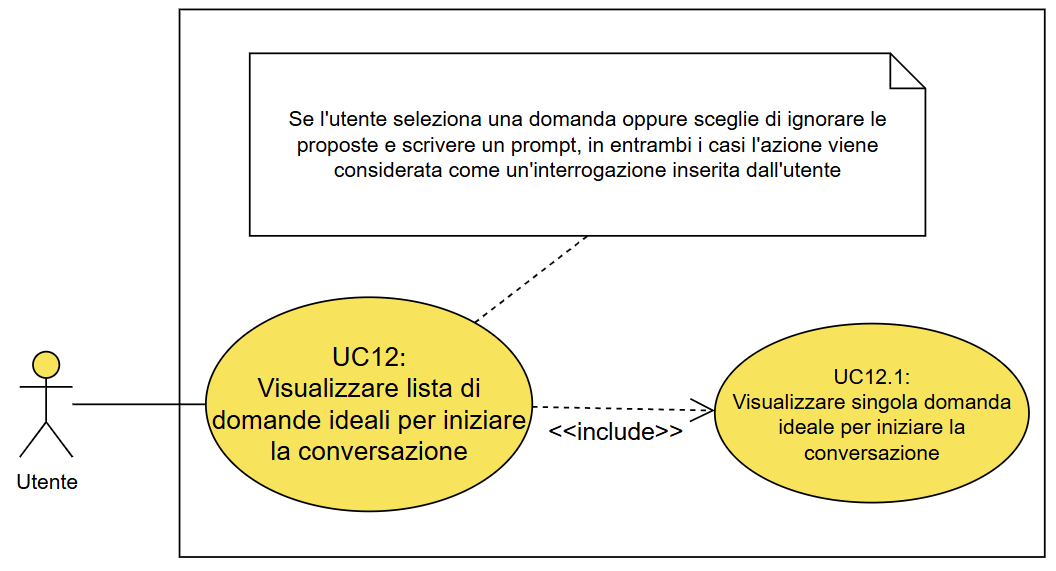
\includegraphics[width=\textwidth]{Diagramma UC12.png}
    \caption{Proporre una lista di domande ideali per iniziare la conversazione}
\end{figure}

\begin{itemize}
    \item \textbf{Attori principali}: Utente;
    \item \textbf{Precondizioni}: L'utente ha appena cominciato una nuova conversazione;
    \item \textbf{Trigger}: L'utente desidera ricevere delle proposte di possibili domande per iniziare la conversazione;
    \item \textbf{Postcondizioni}: L'utente ha ricevuto una serie di domande suggerite dal sistema, che possono essere utilizzate per iniziare la conversazione;
    \item \textbf{Scenario principale}:
    \begin{enumerate}
        \item L'utente avvia l'applicazione;
        \item Il sistema propone una lista di domande ideali per iniziare la conversazione;
        \item L'utente seleziona una delle domande proposte o inserisce una propria domanda.
    \end{enumerate}
    \item \textbf{Sottocasi d'uso}:
    \begin{itemize}
        \item \bulhyperlink{UC12.1}{UC12.1}: Visualizzare una singola domanda ideale per iniziare la conversazione;
    \end{itemize}
\end{itemize}

\hypertarget{UC12.1}{}
\subsubsection{UC12.1: Visualizzare una singola domanda ideale per iniziare la conversazione}

\begin{itemize}
    \item \textbf{Attori principali}: Utente;
    \item \textbf{Precondizioni}: L'utente ha appena cominciato una nuova conversazione;
    \item \textbf{Trigger}: L'utente desidera ricevere una proposta di domanda per iniziare la conversazione;
    \item \textbf{Postcondizioni}: L'utente visualizza una domanda suggerita dal sistema, che può essere utilizzata per iniziare la conversazione;
    \item \textbf{Scenario principale}:
    \begin{enumerate}
        \item L'utente avvia l'applicazione;
        \item Il sistema propone una domanda ideale;
        \item \bulhyperlink{UC1}{UC1}: L'utente seleziona la domanda proposta o inserisce una propria domanda.
    \end{enumerate}
\end{itemize}

\hypertarget{UC14}{}
\subsubsection{UC14: Visualizzare una lista di domande ideali per proseguire la conversazione}

\begin{figure}[h]
    \centering
    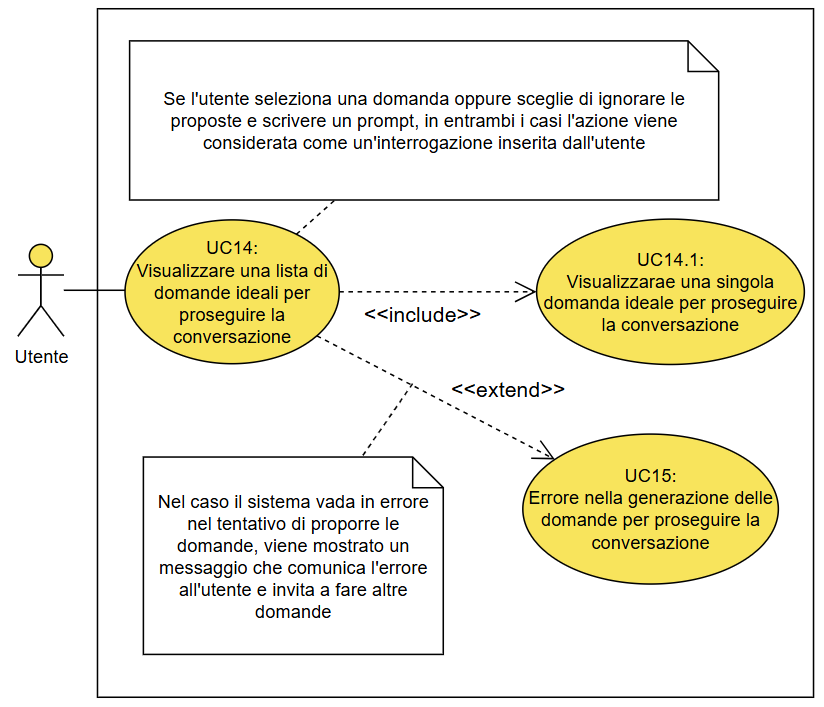
\includegraphics[width=\textwidth]{Diagramma UC14 - UC15.png}
    \caption{\dots}
\end{figure}

\begin{itemize}
    \item \textbf{Attori principali}: Utente;
    \item \textbf{Precondizioni}: L'utente ha appena ricevuto una risposta dal sistema;
    \item \textbf{Trigger}: L'utente desidera ricevere delle proposte di possibili domande per proseguire la conversazione;
    \item \textbf{Postcondizioni}: L'utente ha ricevuto una lista di domande suggerite dal sistema, che possono essere utilizzate per proseguire la conversazione;
    \item \textbf{Scenario principale}:
    \begin{enumerate}
        \item \bulhyperlink{UC5}{UC5}: L'utente ha visualizzato la risposta a una domanda precedente;
        \item Il sistema propone una lista di domande considerate utili rispetto ai messaggi precedenti;
        \item \bulhyperlink{UC1}{UC1}: L'utente seleziona una delle domande proposte o inserisce una propria domanda;
    \end{enumerate}
    \item \textbf{Sottocasi d'uso}:
    \begin{itemize}
        \item \bulhyperlink{UC14.1}{UC14.1}: Visualizzare una singola domanda ideale per proseguire la conversazione.
    \end{itemize}
    \item \textbf{Scenario alternativo}:
    \begin{enumerate}
        \item \bulhyperlink{UC15}{UC15}: Visualizzazione di un messaggio di errore che comunica che il sistema non è in grado di proporre delle domande.
    \end{enumerate}
\end{itemize}

\hypertarget{UC14.1}{}
\subsubsection{UC14.1: Visualizzare una singola domanda ideale per proseguire la conversazione}

\begin{itemize}
    \item \textbf{Attori principali}: Utente;
    \item \textbf{Precondizioni}: L'utente ha appena ricevuto una risposta dal sistema;
    \item \textbf{Trigger}: L'utente desidera ricevere una proposta di domanda per proseguire la conversazione;
    \item \textbf{Postcondizioni}: L'utente visualizza una domanda suggerita dal sistema, che può essere utilizzata per proseguire la conversazione;
    \item \textbf{Scenario principale}:
    \begin{enumerate}
        \item \bulhyperlink{UC5}{UC5}: L'utente ha visualizzato la risposta a una domanda precedente;
        \item Il sistema propone una domanda ideale per proseguire la conversazione;
        \item \bulhyperlink{UC1}{UC1}: L'utente seleziona la domanda proposta o inserisce una propria domanda;
    \end{enumerate}
\end{itemize}

\hypertarget{UC15}{}
\subsubsection{UC15: Errore nella generazione delle domande per proseguire la conversazione}
\begin{itemize}
    \item \textbf{Attori principali}: Utente;
    \item \textbf{Precondizioni}: L'utente ha appena ricevuto una risposta dal sistema;
    \item \textbf{Trigger}: L'utente desidera ricevere delle proposte di possibili domande per proseguire la conversazione;
    \item \textbf{Postcondizioni}: L'utente ha ricevuto un messaggio di errore che comunica che il sistema non è in grado di proporre delle domande;
    \item \textbf{Scenario principale}:
    \begin{enumerate}
        \item \bulhyperlink{UC5}{UC5}: L'utente ha visualizzato la risposta a una domanda precedente;
        \item Il sistema mostra un messaggio di errore che comunica che non è in grado di proporre delle domande.
    \end{enumerate}
\end{itemize}